\subsection{Power}
The systems requires a multitude of supply rails to power the various circuits, this is outlined in figure \ref{fig:power_system}.
\begin{figure}[H]
\centering
\fbox{
\begin{tikzpicture}[node distance = 1cm]
\node [block, fill=\myblue, text width=5em] (caps) {ultra-capacitors};
\node [block, above = 2.5cm of caps, fill=\myred, text width=5em] (USB) {USB power};
\node [block, right = of caps, fill=\myblue, text width=8em] (DCDC) {DC-DC converter \\ (AAT1217)};
\node [block, above right = of DCDC, fill=\myblue, text width=8em] (regulator) {voltage regulator \\ (MCP1703A)};
\node [block, below right = of DCDC, fill=\myblue, text width=8em] (inverter) {voltage inverter \\ (ADM8829)};
\node [block, right = of regulator, fill=\myblue, text width=3em] (filter1) {filter};
\node [block, right = of inverter, fill=\myblue, text width=3em] (filter2) {filter};
\node [block, below = of filter2, fill=\myblue, text width=3em] (filter3) {filter};
%
\path [line, ultra thick] (caps)
	--
	node [anchor = south, align = center]
	{}
	(DCDC);
\path [line, ultra thick, dashed, \myred] (USB)
	-- node [anchor = south, align = center, above right = 0cm and -1cm]
	{\textcolor{black}{provide power to MCU while ultra-capacitors charge}}
	($(USB) + (6.5,0)$)
	to [out = 0, in = 90]
	(regulator);
\path [line, ultra thick] (DCDC)
	to [out = 20, in = -110]
	node [anchor = south, align = center]
	{}
	(regulator);
\path [line, ultra thick] (DCDC)
	to [out = -20, in = 110]
	node [anchor = south, align = center]
	{}
	(inverter);
\path [line, ultra thick] (regulator)
	--
	node [anchor = south, align = center]
	{}
	(filter1);
\path [line, ultra thick] (inverter)
	--
	node [anchor = south, align = center]
	{}
	(filter2);
\path [line, ultra thick] (DCDC)
	to [out = -90, in = 180]
	(filter3);
\path [line, ultra thick] (filter1)
	--
	node [anchor = west, align = center, right = 0.5cm]
	{$+ 3.3 \ \mathsf{V}$}
	($(filter1) + (1.5,0)$);
\path [line, ultra thick] (filter2)
	--
	node [anchor = west, align = center, right = 0.5cm]
	{$\minus 3.3 \ \mathsf{V}$}
	($(filter2) + (1.5,0)$);
\path [line, ultra thick] (filter3)
	--
	node [anchor = west, align = center, right = 0.5cm]
	{${+} 5 \ \mathsf{V}$}
	($(filter3) + (1.5,0)$);
\end{tikzpicture}
}
\caption{Power system architecture.}
\label{fig:power_system}
\end{figure}
%%%%%%%%%%%%%%%%%%%%%%%%%%%%%%%%%%%%%%%%%%%%%%%%%%%%%%%%%%%%%%%%%%%%%%%%%%%%%%%%

\subsubsection{Step-up (boost) converter}
Including a boost converter as the first stage of the power system was a central design decision as it allowed for the entire system (include peripheral circuitry) to continue to operate when the ultra-capacitors were not fully charged. As shown in the systems diagram, all of the supply rails are generated from the switching supply. A Skyworks AAT1217 IC was chosen as it is a high efficiency, synchronous, fixed frequency, step-up converter designed for single-cell or dual-cell battery-powered applications \cite{aat1217}.
\begin{figure}[H]
    \centering
    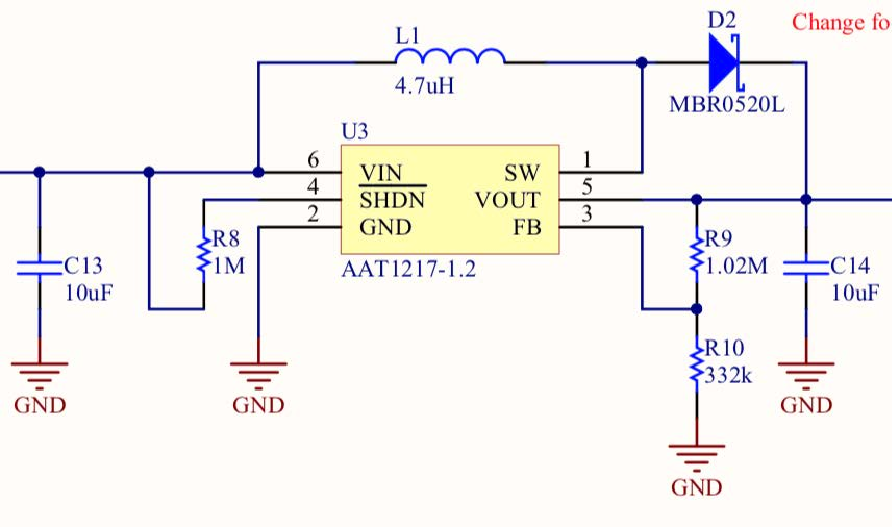
\includegraphics[height = 8cm]{figures/hardware/boost_schematic.pdf}
    \caption{Boost converter schematic excerpt.}
    \label{fig:boost}
\end{figure}
An external Schottky Diode is included since the output voltage exceeds \SI{4.5}{V}, and therefore the internal synchronous rectifier can no longer be used.
\\ \\
A high switching frequency was an important design parameter and was prioritized. Switched mode power supplies are inherently noisy, when the inductor is switched at the operating frequency the circuit will generate noise at the switching frequency and at harmonics of that frequency. This has the potential to radiate and interfere with the sensing circuit. Since the integrity of the state voltages of Cuk Converter is important for the performance of the converter.
\\ \\
To avoid interference, it was important that the Boost Converter operated at a fixed frequency that exceeded that of the \'Cuk Converter and also of the Nyquist rate of the ADC. Therefore, by choosing a boost converter that had a switching frequency that exceed that of the Anti-Aliasing filter ensured that the noise was not present in the sensed signals. The AAT1217 operates at a fixed frequency of 1.2MHz, this well exceeds the switching frequency of the \'Cuk converter.
\\ \\
Choosing the current rating of the boost converter was another important design constraint. This was a difficult specification to quantify as it varied with the input and output voltages of the converters.
\\ \\
A Boost converter topology was chosen as it allowed for the power to be stepped-up to a higher voltage will still being able to operate at the supply voltages. Due to the way that the charge controller (LTC4425) the ultra-capacitor stack will always be charged to slightly lower than the \SI{5}{V} output is specified. Hence the input to the boost converter will always be less than its fixed output of \SI{5}{V}.
%%%%%%%%%%%%%%%%%%%%%%%%%%%%%%%%%%%%%%%%%%%%%%%%%%%%%%%%%%%%%%%%%%%%%%%%%%%%%%%%

\subsubsection{Linear regulator}
Several devices, including the microcontroller require a nominal \SI{3.3}{V} to operate therefore a Linear Voltage Regulator was used to drop the 5V output from the boost converter down to \SI{3.3}{V}. The Microcontroller MCP1073A \SI{250}{mA}, \SI{16}{V}, Low Quiescent Current LDO Regulator was chosen.
\begin{figure}[H]
    \centering
    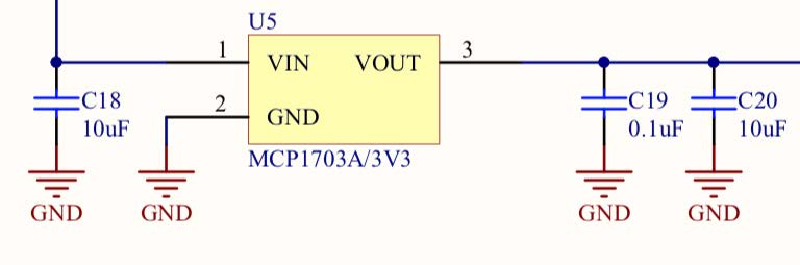
\includegraphics[width = 12cm]{figures/hardware/regulator_schematic.pdf}
    \caption{Linear regulator converter schematic excerpt.}
    \label{fig:regulator}
\end{figure}
To allow for flexibility in power supply design, the linear regulator was chosen such that it had a wide operating range. Allowing for a \SI{9}{V} DC supply to be used as a backup, in the event that USB charging option didn’t meet up performance criteria. The MCP1073A supports input voltages up to \SI{16}{V}. Additionally this allow the ultra-capacitors to be bypassed completely, allowing for operation directly was the \SI{9}{V} dc supply.

\paragraph{Power supply rejection ratio (PSRR) and output noise}
Since the \SI{3.3}{V} voltage rail would be used to supply the analog components of the system, this included the ADC and the op amps used to sense the input and output for the controller. As a switching power supply was used to maintain a constant \SI{5}{V} across most of its capacity, this supply rail was inherently noisy. To maintain a clean DC voltage on the supplies of these sensitive analog components it was important to consider the power supply rejection ratio of the LDO \cite{supply_ripple}.
\\ \\
The MCP1703A LDO Regulator has a PSRR below $-\SI{50}{dB}$ for frequencies above \SI{1}{MHz} (\SI{200}{mV} of ripple) \cite{mcp1703a}. As the switching frequency of the Boost Converter is typically \SI{1.2}{MHz} this will assist in producing a clean DC supply voltage for the analog circuitry.
%%%%%%%%%%%%%%%%%%%%%%%%%%%%%%%%%%%%%%%%%%%%%%%%%%%%%%%%%%%%%%%%%%%%%%%%%%%%%%%%
\subsubsection{Voltage inverter}
Since the \'Cuk Converter topology produces an inverted output the op amps used in the sensing circuitry must use dual supplies. The ADN8829 Switched-Capacitor Voltage Inverter is used in conjunction with the LDO regulator to produce $\pm\SI{3.3}{V}$ supply rails for the op amps.
\begin{figure}[H]
    \centering
    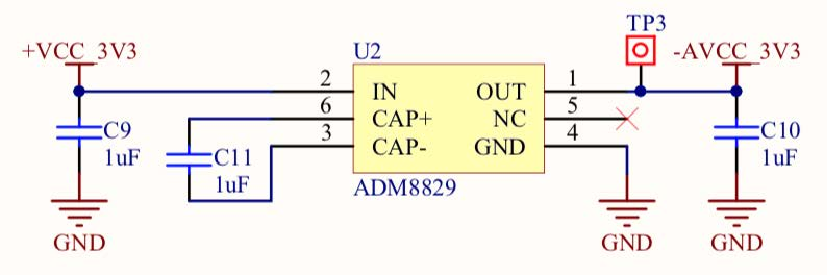
\includegraphics[width = 12cm]{figures/hardware/inverter_schematic.pdf}
    \caption{Voltage inverter schematic excerpt.}
    \label{fig:inverter}
\end{figure}
It was identified that a switched capacitor technique would be employed to generate the negative voltage as it was cost effective and had required little redesign to include. Due to a misunderstanding of the operation of the \'Cuk Converter, most of the hardware was designed before (including the sensing circuity) a negative supply was identified as a requirement. Therefore, the easy of integration was important to not delay the prototype further.
\\ \\
The ADM8829 was chosen as it was designed to be used for op amp supply rails and required minimal additional components. The recommended input and output capacitors were already included in the bill of materials, reducing design time. 
\\ \\
Switch capacitor converters, not unlike boost converters, are inherently noisy. By varying which terminal of the external capacitor is connected to ground periodically, a negative voltage is generated. This produces a significant ripple on the output which must be filtered to avoid corrupting the measurements made by the sensing circuitry. The Charge-Pump Frequency is typically \SI{120}{kHz}. This is close to the operating frequency of the \'Cuk Converter, consequently care must be take such that this does not interfere with the measures made by the sensing circuitry. Output ripple can vary between \SI{25}{mV} to \SI{130}{mV} peak-peak \cite{adm8829}, which when the sensed voltages are scaled by the resistive dividers will be of the same order of magnitude. In the next section the circuitry used to attenuate most of the ripple was outline. In future designs this particular chip would not be used and one with a much higher frequency would be used, however lost cost charge pump circuits in the MHz are rare. 
\\ \\
Produces \SI{25}{mA} of output current which is more than enough to supply the op amps. Include reference to calculations. However it is vital that the $-\SI{3.3}{V}$ power rail is not routed near any of the sense lines as this would interfere with the \'Cuk Converter which is switching at a similar frequency.
%%%%%%%%%%%%%%%%%%%%%%%%%%%%%%%%%%%%%%%%%%%%%%%%%%%%%%%%%%%%%%%%%%%%%%%%%%%%%%%%